\documentclass[12pt, a4paper]{article}

\usepackage[utf8]{inputenc}
\usepackage{amsmath}
\usepackage{amssymb}
\usepackage{graphicx}
\usepackage{geometry}
\usepackage{hyperref}
\usepackage{float}
\usepackage{caption}
\usepackage{subcaption}
\usepackage{fancyhdr}
\usepackage{siunitx}
\usepackage{multirow}

\bibliographystyle{ieeetr}

\geometry{
	a4paper,
	total={170mm,257mm},
	left=20mm,
	top=20mm,
}

\pagestyle{fancy}
\fancyhf{}
\fancyhead[L]{\textit{Adaptive Hybrid Control Error for Vehicle Platoons via Reinforcement Learning}}
\fancyhead[R]{30/03/2026}
\fancyfoot[C]{\thepage}
\setlength{\headheight}{15pt}

\hypersetup{
	colorlinks=true,
	linkcolor=blue,
	citecolor=black,
	filecolor=magenta,
	urlcolor=cyan,
	pdftitle={\textit{Adaptive Hybrid Control Error for Vehicle Platoons via Reinforcement Learning}},
	pdfpagemode=FullScreen,
}

\title{
	\vspace{2cm}
	
\includegraphics[width=0.3\textwidth]{images/logo.png}
	\vspace{1cm}
	
	\textbf{Adaptive Hybrid Control Error for Vehicle Platoons via Reinforcement Learning} \\
	\vspace{0.4cm}
	Mid-Report \\
	\vspace{1cm}
}

\author{
	\textbf{Authors:}\\
	Mustafa Kamal\\
	Rafael Maestre López\\
	Charelle Khoury\\[1.5cm]
	%\textbf{Institution:}\\
	%[Institution Name]\\[0.8cm]
	\textbf{Course:}\\
	Project S8 - P22\\[0.8cm]
	%\textbf{Course Year:}\\
	%2026
}

\date{}

\begin{document}
	
	\hypersetup{pageanchor=false}
	\maketitle
	\thispagestyle{empty} % no page number on title page
	
	% --- Table of contents (Roman numerals) ---
	\newpage
	\pagenumbering{roman}
	\setcounter{page}{1}
	
	\tableofcontents
	\newpage
	
	% --- Main content (Arabic, starting at 1) ---
	\hypersetup{pageanchor=true}
	\pagenumbering{arabic}
	\setcounter{page}{1}
	
	\section{Introduction}

\subsection{A Short Description}
The modernization of intelligent transportation systems (ITS) has necessitated a paradigm shift from individual vehicle autonomy to cooperative automation. Vehicular platooning offers a promising solution to traffic congestion, fuel inefficiency, and road safety. 

Thus, our work motivates an "Adaptive Hybrid Control strategy" using RL to adjust the weight between micro and macro. This transition from the standard Adaptive Cruise Control (ACC) to Cooperative Adaptive Cruise Control (CACC) introduces challenges in string stability, the ability to attenuate disturbances, especially under communication delays.

\subsection{Motivation}
A recurring difficulty in platoon control is the trade-off between robustness and anticipation:
\begin{itemize}
    \item \textbf{Local sensing:} Radar/LiDAR-based control is robust to communication failures and is well suited to collision avoidance, but it often struggles to damp disturbances once they propagate through a long platoon.
    \item \textbf{Global cooperation:} Leader or platoon-wide information can improve string stability, but its benefits deteriorate quickly when communication is delayed, intermittent, or noisy.
\end{itemize}


\subsection{Our contributions}
\begin{itemize}
    \item A mixed-traffic ring-road model combining SIDM-based HDVs, ACC/CTH-based CAVs, and mesoscopic traffic indicators derived from upstream flow.
    \item A layered control architecture in which a rule-based mesoscopic headway adaptation is refined by a residual RL policy, rather than replaced by a fully learned controller.
    \item A corrected and admissible evaluation protocol at 50\,\% human penetration, leading to the first clean comparison in this project between the no-RL baseline, PPO, and SAC.
\end{itemize}

	
	\section{Traffic Environment}

\subsection{Driver Models}
\subsubsection{Intelligent Driver Model (IDM)}

The Intelligent Driver Model (IDM) is a deterministic microscopic car-following model describing the longitudinal dynamics of vehicle $i$ as a function of its own velocity, the spacing to its predecessor, and their relative velocity \cite{Treiber.2000}. The acceleration of vehicle $i$ is defined as

\begin{equation}
	\dot{v}_i =
	a_{max} \left[
	\underbrace{1 - \left( \frac{v_i}{v_d} \right)^{\delta}}_{\text{free-road acceleration}}
	-
	\underbrace{\left( \frac{s^*(v_i,\Delta v_i)}{s_i} \right)^2}_{\text{interaction (braking) term}}
	\right].
\end{equation}
Here $v_i$ is the ego velocity, $v_d$ the desired free-flow velocity, $a_{max}$ the maximum acceleration, $b$ the desired deceleration, and $\delta$ the acceleration exponent \cite{Treiber.2000}. The free-road term drives the vehicle toward $v_d$, while the interaction term enforces deceleration when the actual spacing $s_i$ falls below the desired spacing $s^*$.


The spacing is defined as
\begin{equation}
	s_i = x_{i-1} - x_i - L,
\end{equation}

where $x_i$ and $x_{i-1}$ denote the longitudinal positions of vehicle $i$ and its leader, respectively, and $L$ is the vehicle length. The relative velocity is defined as $\Delta v_i = v_i - v_{i-1}$.

The desired dynamic spacing is given by

\begin{equation}
	s^*(v_i,\Delta v_i)
	=
	\underbrace{s_0}_{\text{jam distance}}
	+
	\underbrace{v_i T_H}_{\text{time-headway term}}
	+
	\underbrace{\frac{v_i \Delta v_i}{2 \sqrt{a_{max} b}}}_{\text{anticipation term}}.
\end{equation}
The terms represent the jam distance $s_0$, the time-headway policy $v_i T_H$, and an anticipative braking correction \cite{Treiber.2000}.


\subsubsection{Stochastic Intelligent Driver Model (SIDM)} \label{SIDM}

To account for perception errors, behavioral variability, and unmodeled disturbances, the IDM can be extended by introducing a stochastic acceleration component \cite{Treiber.2018}. The stochastic IDM (SIDM) is formulated as

\begin{equation}
	\dot{v}_i =
	\underbrace{f(s_i, v_i, v_{i-1})}_{\text{deterministic IDM}}
	+
	\underbrace{\xi_i(t)}_{\text{stochastic acceleration noise}},
\end{equation}

where $f(\cdot)$ denotes the deterministic IDM acceleration function and $\xi_i(t)$ is a stochastic process representing white acceleration noise.

The stochastic term satisfies
\begin{equation}
	\langle \xi_i(t) \rangle = 0,
\end{equation}
\begin{equation}
	\langle \xi_i(t)\xi_j(t') \rangle
	=
	Q \, \delta_{ij} \, \delta(t - t'),
\end{equation}

where $Q$ denotes the noise intensity, $\delta_{ij}$ is the Kronecker delta ensuring independence between different vehicles, and $\delta(t-t')$ is the Dirac delta distribution representing temporal white noise \cite{Treiber.2018}.

 Close to the string stability threshold, noise can generate spatiotemporal correlations and traffic oscillations resembling stop-and-go waves. Consequently, the SIDM provides a unified framework for analyzing deterministic instabilities and noise-induced traffic dynamics \cite{Treiber.2018}.

\subsubsection{Connected Autonomous Vehicle (CAV) Model}\label{CAV}

For connected autonomous vehicles, we adopt the point-mass longitudinal dynamics described in \cite{Mirabilio.2023}. The motion of vehicle $i$ is governed by

\begin{equation}
\dot{x}_i = v_i,
\qquad
\dot{v}_i = u_i,
\end{equation}
In a car-following configuration, the spacing and relative velocity are defined as
\begin{equation}
s_i = x_{i-1} - x_i - L,
\qquad
\Delta v_i = v_i - v_{i-1}.
\end{equation}

CAVs implement an Adaptive Cruise Control (ACC) strategy based on a Constant Time Headway (CTH) policy. The desired spacing is given by
\begin{equation}
s_i^{\mathrm{ref}} = s_0 + T_C v_i,
\end{equation}

where $s_0$ denotes the standstill spacing and $T_C > 0$ is the selected time headway.

Defining the spacing error
\begin{equation}
e_{p,i} = s_i - s_i^{\mathrm{ref}},
\end{equation}

its dynamics follow from
\begin{equation}
\dot{s}_i = -\Delta v_i,
\qquad
\dot{s}_i^{\mathrm{ref}} = T_C \dot{v}_i = T_C u_i,
\end{equation}

which yields
\begin{equation}
\dot{e}_{p,i} = -\Delta v_i - T_C u_i.
\end{equation}

A linear ACC controller that regulates both spacing and velocity errors can therefore be written as
\begin{equation}
u_i =
k_s ( s_i - s_i^{\mathrm{ref}} )
-
k_v \Delta v_i,
\end{equation}

where $k_s > 0$ and $k_v > 0$ denote the spacing and velocity feedback gains, respectively. This control law constitutes a linear realization of the CTH policy and is consistent with the mesoscopic ACC formulation proposed in \cite{Mirabilio.2023}.

An important property of the CTH-based ACC strategy is its capability to guarantee weak string stability using only local measurements \cite{Swaroop.2001}. In the frequency domain, the disturbance propagation transfer function satisfies
\begin{equation}
\| H(j\omega) \|_{\infty} \le 1,
\end{equation}
ensuring that spacing disturbances are not amplified upstream along a vehicle string.
Moreover, robustness with respect to sensing and actuation delays imposes a constraint on the admissible implementation lag. In particular, the total delay must satisfy
\begin{equation}
T_C \le \frac{h_w}{2},
\end{equation}
indicating that allowable delay is directly limited by the chosen time headway \cite{Swaroop.2001}.

\subsection{Mixed Traffic Model}

We consider a mixed traffic system composed of $N$ vehicles circulating on a single-lane ring road of length $L_{\mathrm{ring}}$. The vehicle indices satisfy periodic boundary conditions such that vehicle $1$ follows vehicle $N$.

Let $x_i(t)$ and $v_i(t)$ denote the position and velocity of vehicle $i \in \{1,\dots,N\}$. The ring-road constraint is given by
\begin{equation}
x_{i-1}(t) > x_i(t), 
\qquad
x_0(t) := x_N(t) + L_{\mathrm{ring}}.
\end{equation}

The spacing is defined as
\begin{equation}
s_i = x_{i-1} - x_i - L,
\end{equation}
where periodicity applies for $i=1$.

Let $\mathcal{H}$ denote the set of HDVs and $\mathcal{C}$ the set of CAVs, with penetration rate
\begin{equation}
P = \frac{|\mathcal{C}|}{N}.
\end{equation}

\vspace{0.5cm}

Human-driven vehicles are modeled according to the stochastic Intelligent Driver Model introduced in Subsection~\ref{SIDM}.

HDVs do not utilize acceleration information of the preceding vehicle, reflecting the absence of communication capabilities. Furthermore, HDVs are characterized by a larger effective reaction time $T_H$, representing the delay associated with human perception and actuation. Consequently, their response to traffic perturbations is slower and more susceptible to amplification of stochastic fluctuations.

\vspace{0.5cm}

Connected autonomous vehicles are modeled according to the ACC framework introduced previously in \ref{CAV}. In contrast to HDVs, CAVs are assumed to exhibit higher sensitivity coefficients and a shorter desired time headway $T_C$, reflecting their faster sensing \cite{Gong.2024}. The condition $T_C < T_H$ therefore captures the higher responsiveness of CAVs compared to HDVs.

When a CAV follows an HDV, communication-based acceleration information is unavailable. In this degraded configuration, the feedforward gain is set to $k_a = 0$, and the effective time headway is increased to $T_C^{\mathrm{deg}} > T_C$, representing reduced cooperative capability. This modeling choice captures the performance degradation of CAVs in mixed traffic reported in \cite{Gong.2024} and \cite{Cen.2025}.

\vspace{0.5cm}

The closed-loop mixed system is therefore
\begin{equation}
\dot v_i =
\begin{cases}
f_{\mathrm{IDM}}(s_i, v_i, v_{i-1}) + \xi_i(t),
& i \in \mathcal{H}, \\[6pt]
k_s ( s_i - s_i^{\mathrm{ref}} )
- k_v \Delta v_i
+ k_a a_{i-1},
& i \in \mathcal{C}.
\end{cases}
\end{equation}

\subsection{Macroscopic Information}

Up to this point, only microscopic vehicle interactions have been considered. To improve the performance of the proposed framework, macroscopic traffic information are introduced according to \cite{Mirabilio.2023}. In particular, we define the mean velocity on the ring as
\begin{equation}
\bar v(t) = \frac{1}{N} \sum_{i=1}^{N} v_i(t),
\end{equation}
and the velocity variance
\begin{equation}
\sigma_v^2(t)
=
\frac{1}{N}
\sum_{i=1}^{N}
\left( v_i(t) - \bar v(t) \right)^2.
\end{equation}

The mean velocity represents the macroscopic traffic state, while the variance quantifies the level of speed dispersion and therefore the intensity of oscillations. As discussed in \cite{Mirabilio.2023}, the variance provides a compact indicator of transient traffic behavior and string instability.



	
	\section{Reinforcement Learning}

In this project, reinforcement learning (RL) is used to improve the behavior of connected and automated vehicles (CAVs) in mixed traffic. The main idea is not to replace the baseline controller, but to add an adaptive layer on top of it. This learned layer adjusts the time headway policy according to the current traffic situation. In this way, the controller keeps its physical interpretation while gaining the ability to react to complex traffic patterns that are difficult to model explicitly.

\subsection{Fundamentals}

The RL problem is formulated as a Markov Decision Process (MDP),
\[
\mathcal{M} = (\mathcal{S}, \mathcal{A}, P, r),
\]
where $\mathcal{S}$ is the state space, $\mathcal{A}$ is the action space, $P$ represents the traffic dynamics, and $r$ is the reward.

At each time step, the agent observes the traffic state, selects an action, applies it to the controller, and receives a reward. In the current implementation, the state of each CAV $i$ is defined as
\[
x_i =
(\mu_{v,i}, \sigma_{v,i}^2, \delta^{\mathrm{macro}}_{v,i}, v_i, s_i, \Delta v_i, a_{\ell(i)}, \alpha_i^{prev}),
\]
where $\mu_{v,i}$ and $\sigma_{v,i}^2$ are the upstream mean velocity and velocity variance, $\delta^{\mathrm{macro}}_{v,i}=v_i-\mu_{v,i}$ is the speed mismatch with the local upstream flow, $v_i$ is the ego speed, $s_i$ is the spacing to the leader, $\Delta v_i$ is the relative speed, $a_{\ell(i)}$ is the leader acceleration, and $\alpha_i^{prev}$ is the previously applied headway scaling factor.

This state combines \emph{microscopic} information, such as spacing and relative velocity, with \emph{mesoscopic} information, such as the average speed and speed variance of upstream traffic. This is important because local measurements alone may not be enough to detect the development of traffic waves.

The action is a residual correction of the headway scaling:
\[
\mathcal{A} = \{\Delta\alpha_i \in [-\Delta\alpha_{\max}, +\Delta\alpha_{\max}]\}.
\]
The final headway scaling factor is then given by
\[
\alpha_i(t) =
\mathrm{clip}\left(\alpha_i^{rule}(t) + \Delta\alpha_i(t)\right),
\]
where $\alpha_i^{rule}(t)$ is the baseline headway scaling provided by the rule-based mesoscopic module. Therefore, RL only refines the baseline decision instead of replacing it. The learned policy can be written as
\[
\pi : \mathcal{S} \rightarrow \mathcal{A},
\qquad \Delta\alpha_i(t) = \pi(x_i(t)).
\]

\subsection{Reward design}

The reward is designed to stay aligned with the engineering goals of the project rather than with a purely numerical score:
\[
r_t = r_{\mathrm{sf}} + r_{\mathrm{sp}} + r_{\mathrm{ef}} + r_{\mathrm{cf}} + r_{\mathrm{ss}} + r_{\sigma^2}.
\]

For the spacing-regulation term, the controller uses the desired gap
\[
s_i^{\mathrm{des}}[t] = d_0 + h_i'[t]\,v_i[t],
\]
and the tracking error
\[
e_i[t] = s_i[t] - s_i^{\mathrm{des}}[t].
\]

The different reward terms have a clear physical meaning:
\begin{itemize}
    \item $r_{\mathrm{sf}}$: safety term, penalizing unsafe spacing and too small time headway;
    \item $r_{\mathrm{sp}}$: spacing regulation term, encouraging tracking of the desired spacing;
    \item $r_{\mathrm{ef}}$: efficiency term, encouraging the vehicle speed to remain close to the upstream mean speed;
    \item $r_{\mathrm{cf}}$: comfort term, penalizing high jerk;
    \item $r_{\mathrm{ss}}$: string stability term, penalizing amplification of spacing errors along the platoon;
    \item $r_{\sigma^2}$: traffic smoothness term, penalizing large velocity variance in the traffic stream.
\end{itemize}

Taken together, these terms encourage a policy that is safe first, but also smooth and useful at traffic scale. A controller that improved one vehicle while making the overall flow worse would not be acceptable here.

\subsection{PPO}

Proximal Policy Optimization (PPO) is a policy-gradient RL algorithm that updates the policy in a stable and conservative way. Its main advantage is that it is simple to implement and usually robust during training. PPO avoids large policy updates by using a clipped objective:
\[
L^{\mathrm{PPO}}(\theta)
=
\mathbb{E}_t
\left[
\min\left(
r_t(\theta)\hat{A}_t,\;
\mathrm{clip}(r_t(\theta),1-\epsilon,1+\epsilon)\hat{A}_t
\right)
\right],
\]
where
\[
r_t(\theta)=\frac{\pi_\theta(a_t|s_t)}{\pi_{\theta_{\mathrm{old}}}(a_t|s_t)},
\]
and $\hat{A}_t$ is the estimated advantage. In this project, PPO mainly serves as a strong baseline: it is simple to implement, reasonably stable, and easy to interpret when comparing learning behavior across runs.

\subsection{SAC}

Soft Actor-Critic (SAC) is another RL algorithm for continuous control. Unlike PPO, SAC is an off-policy method and includes an entropy term in its objective:
\[
J(\pi)
=
\sum_t
\mathbb{E}
\left[
r(s_t,a_t) + \beta \mathcal{H}(\pi(\cdot|s_t))
\right],
\]
where $\mathcal{H}(\pi(\cdot|s_t))$ is the policy entropy and $\beta$ controls the exploration level.

SAC is well suited to continuous-action problems and stochastic environments. Its replay buffer allows reuse of past experience, which can improve sample efficiency compared with on-policy methods such as PPO. This makes it a natural alternative here because the action is continuous and the mixed-traffic environment is noisy due to stochastic HDV behavior.

\subsection{Role of RL in the framework}

In our setup, RL does not produce the full acceleration command. It only adjusts the headway scaling around a rule-based mesoscopic baseline. This design choice is deliberate: it keeps the controller interpretable, limits unsafe departures from a known operating point, and makes it easier to judge whether learning is adding value beyond the handcrafted adaptation.

	
	\section{System Architecture}

The proposed controller is organized as a layered architecture that combines a conventional vehicle-level controller with mesoscopic traffic awareness. Figure~\ref{fig:system_architecture} summarizes the four layers: simulation, perception, adaptation, and control.

\begin{figure}[!htbp]
    \centering
    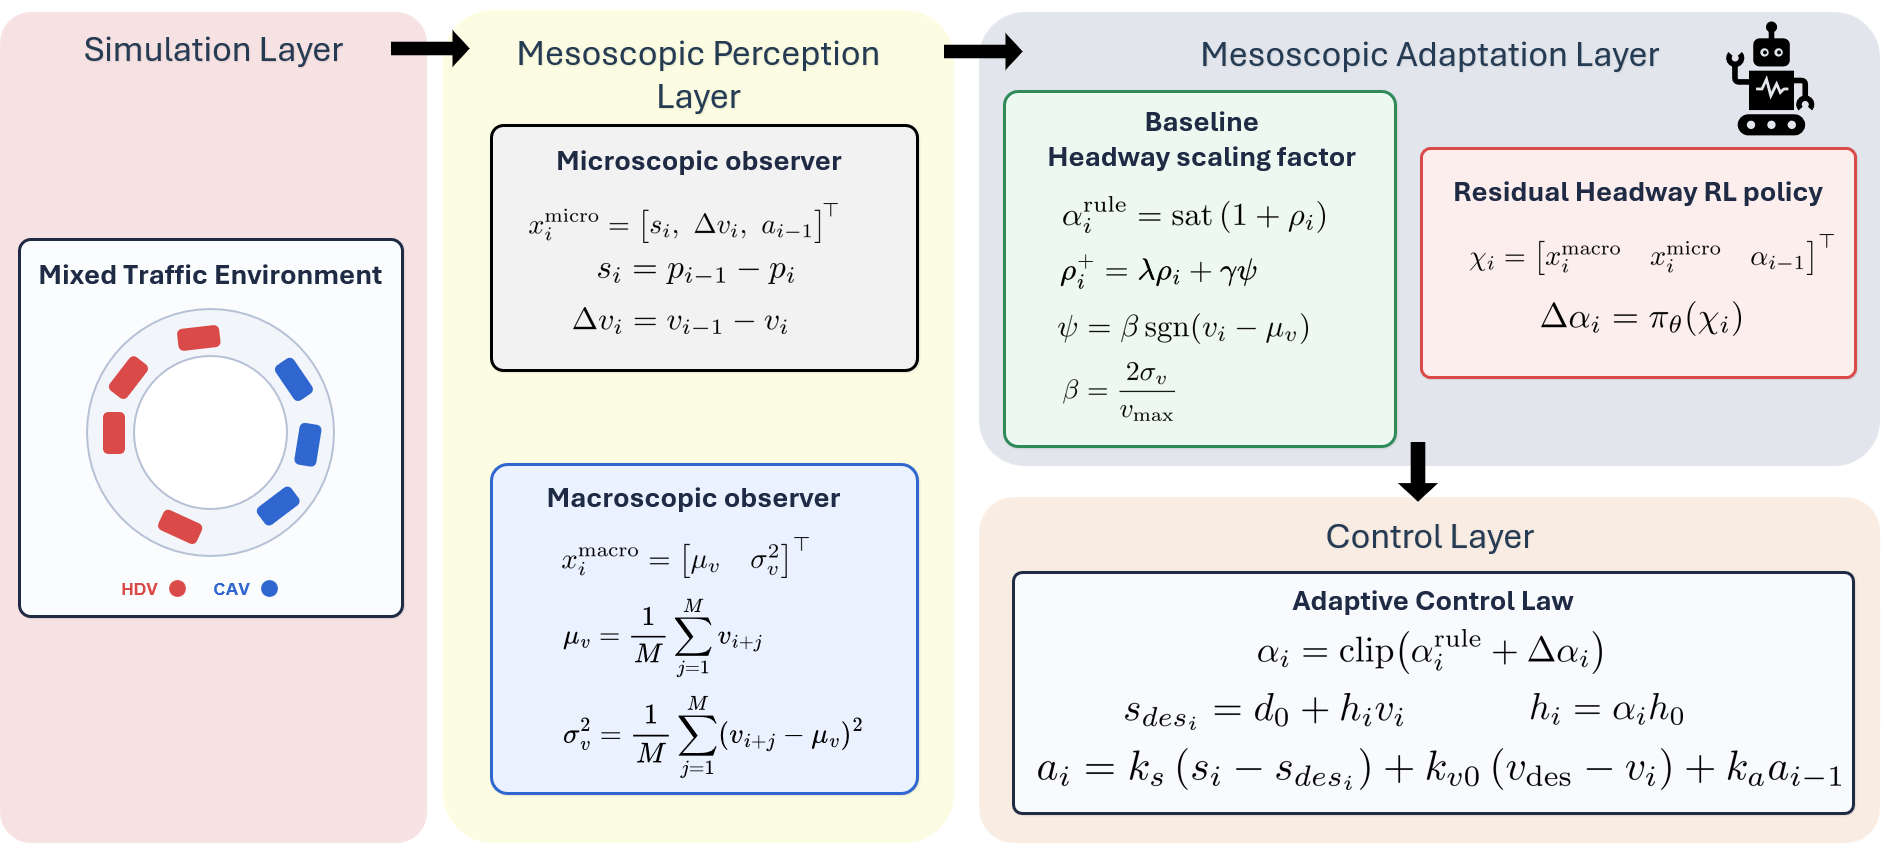
\includegraphics[width=\textwidth]{images/system_architecture.png}
    \caption{Overview of the proposed system architecture.}
    \label{fig:system_architecture}
\end{figure}

\subsection{Overall structure}

At each simulation step, the environment updates all vehicles, the perception layer summarizes the local and upstream traffic state, the adaptation layer converts those observations into a headway adjustment, and the control layer applies the resulting acceleration command. Separating these roles makes the framework easier to debug and makes it explicit what the RL block is allowed to change.

\subsection{Simulation layer}

The simulation layer models a single-lane ring road where HDVs and CAVs coexist. The ring-road setting removes open-boundary entry and exit effects, which makes the appearance of stop-and-go waves easier to observe and compare across methods. This layer provides the positions, velocities, spacing, and leader-acceleration signals used by the upper layers.

\subsection{Mesoscopic perception layer}

The perception layer extracts the information used by the controller. It contains two complementary observers.

\paragraph{Microscopic observer.}
The microscopic observer describes the local car-following situation of vehicle $i$. It uses the spacing, relative velocity, and ego speed:
\[
x_i^{\mathrm{micro}} =
\begin{bmatrix}
s_i & \Delta v_i & a_{i-1}
\end{bmatrix}^{\top},
\]
with
\[
s_i = p_{i-1} - p_i,
\qquad
\Delta v_i = v_{i-1} - v_i.
\]
These variables describe the immediate interaction with the preceding vehicle and are the standard quantities used by longitudinal controllers.

\paragraph{Macroscopic observer.}
The second observer captures collective traffic behavior upstream of the CAV. Instead of looking only at the leader, it summarizes the traffic state over a perception horizon. The two main quantities are the upstream mean velocity and the upstream velocity variance:
\[
x_i^{\mathrm{macro}} =
\begin{bmatrix}
\mu_v & \sigma_v^2
\end{bmatrix}^{\top},
\]
with
\[
\mu_v = \frac{1}{M}\sum_{j=1}^{M} v_{i+j},
\qquad
\sigma_v^2 = \frac{1}{M}\sum_{j=1}^{M}(v_{i+j}-\mu_v)^2.
\]
The mean velocity gives an estimate of the average upstream traffic speed, while the variance indicates how irregular or unstable the traffic stream is.

\subsection{Mesoscopic adaptation layer}

The adaptation layer transforms the observed traffic information into a headway modification for the CAV controller. It contains two parts: a baseline adaptive headway mechanism and a residual reinforcement learning policy.

\paragraph{Baseline adaptive headway.}
The baseline mechanism computes a rule-based headway scaling factor from the macroscopic traffic information. The update can be written as
\[
\alpha_i^{\mathrm{rule}} = \mathrm{sat}(1+\rho_i),
\]
with the internal state
\[
\rho_i^{+} = \lambda \rho_i + \gamma \psi,
\]
and the perception signal
\[
\psi = \beta \,\mathrm{sgn}(v_i-\mu_v),
\qquad
\beta = \frac{2\sigma_v}{v_{\max}}.
\]
This mechanism has a simple interpretation. When upstream traffic becomes more variable, the controller increases the effective headway in order to react more cautiously. When traffic is smoother, the headway can be reduced. The filtering through $\rho_i$ also avoids abrupt parameter changes.

\paragraph{Residual RL policy.}
On top of the baseline adaptation, a residual policy computes a correction term:
\[
\chi_i =
\begin{bmatrix}
    \mu_v & \sigma_v^2 & (v_i-\mu_v) & v_i & s_i & \Delta v_i & a_{i-1} & \alpha_i^{prev}
\end{bmatrix}^{\top},
\qquad
\Delta \alpha_i = \pi_{\theta}(\chi_i).
\]
The role of this block is to refine the rule-based decision without changing the overall structure of the controller. In other words, the adaptive law remains physically interpretable, while the learning block adds flexibility when the traffic situation becomes more complex. The resulting policy input therefore combines mesoscopic information, local car-following variables, and the previously applied headway state in a single 8-dimensional vector.

\subsection{Control layer}

The control layer converts the adapted headway into a longitudinal acceleration command for the CAV. The final scaling factor is
\[
\alpha_i = \mathrm{clip}\!\left(\alpha_i^{\mathrm{rule}} + \Delta \alpha_i\right),
\]
and the corresponding time headway becomes
\[
T_i = \alpha_i T_0.
\]
This adapted headway is then used inside the microscopic CACC/CTH controller:
\[
a_i = k_s\left(s_i - d_0 - T_i v_i\right)
      + k_v \Delta v_i
      + k_a a_{i-1}
      + k_{v0}(v_{\mathrm{des}} - v_i).
\]

The lower-level controller therefore remains a standard feedback law; the upper layers only adapt the time-headway parameter used inside it. This separation preserves a clear physical interpretation of the final command.

	
	\section{Current Progress, Results and Perspectives}

This section reports the state of the consolidated implementation after the first report draft. From this point onward, the project is presented as a single main codebase. The experiments below correspond to the current pipeline only: the same residual RL controller, the same mesoscopic adaptation mechanism, and the same evaluation scripts used to produce the latest local results.

\subsection{What was added after the first draft}

Several substantial changes were applied after the initial report version and before the final experiments presented here:
\begin{itemize}
    \item the missing evaluation metrics were integrated into the main pipeline, in particular the late-run objective $\texttt{mean\_speed\_last100}$, string-stability validity flags, collision-clamp counts, and safety-constraint summaries;
    \item a checkpoint-aware early-stopping monitor was introduced, together with best-model restoration and explicit summaries of the best observed training point;
    \item the training loop was rewritten into a vectorized PyTorch backend able to batch several environments at once and run on GPU while keeping the same 8-feature observation format used by the main controller;
    \item the report-generation scripts were hardened so that evaluation outputs now include the effective configuration and the comparison report no longer breaks when a metric is unavailable or invalid.
\end{itemize}

These updates were not only implementation cleanups. After they were applied, additional training and evaluation runs were launched again, so the results reported below correspond to the updated pipeline rather than to the earlier draft state.

\subsection{Experimental protocol used for the updated results}

The updated experiments were run on the CentraleSup\'elec DCE infrastructure with a CUDA-enabled PyTorch environment and an NVIDIA RTX~2080~Ti GPU. The GPU acceleration was used for training only; the evaluation runs still use the standard simulation path so that the learned models are tested in the same operational setting as the controller used at inference time.

The final experimental campaign contains:
\begin{itemize}
    \item two training runs: one PPO run and one SAC run, both at 50\,\% human-driver ratio;
    \item 200 physical training episodes per algorithm;
    \item 8 parallel environments during training, which means that each 200-episode run is executed as 25 vectorized training batches;
    \item nine evaluation runs in total: No~RL, PPO, and SAC, each tested at 25\,\%, 50\,\%, and 75\,\% human-driver ratios.
\end{itemize}

The evaluation focuses on the metrics that are the most informative for this project: late-run mean speed, late-run speed variance, comfort, minimum gap, collision warnings, collision clamps, and the validity of the string-stability experiment.

\subsection{Training summary}

Table~\ref{tab:training_summary_updated} summarizes the two updated training runs. The important point is that the best observed training point appears early for both algorithms, whereas the final checkpoint is not the best one in terms of variance minimization.

\begin{table}[!htbp]
\centering
\caption{Training summary for the updated GPU-enabled pipeline.}
\label{tab:training_summary_updated}
\small
\begin{tabular}{lccccc}
\hline
Method & Physical episodes & Batches & Best batch & Best variance & Final variance \\
\hline
PPO & 200 & 25 & 9 & 1.471 & 1.877 \\
SAC & 200 & 25 & 3 & 1.530 & 1.762 \\
\hline
\end{tabular}
\end{table}

\begin{figure}[!htbp]
    \centering
    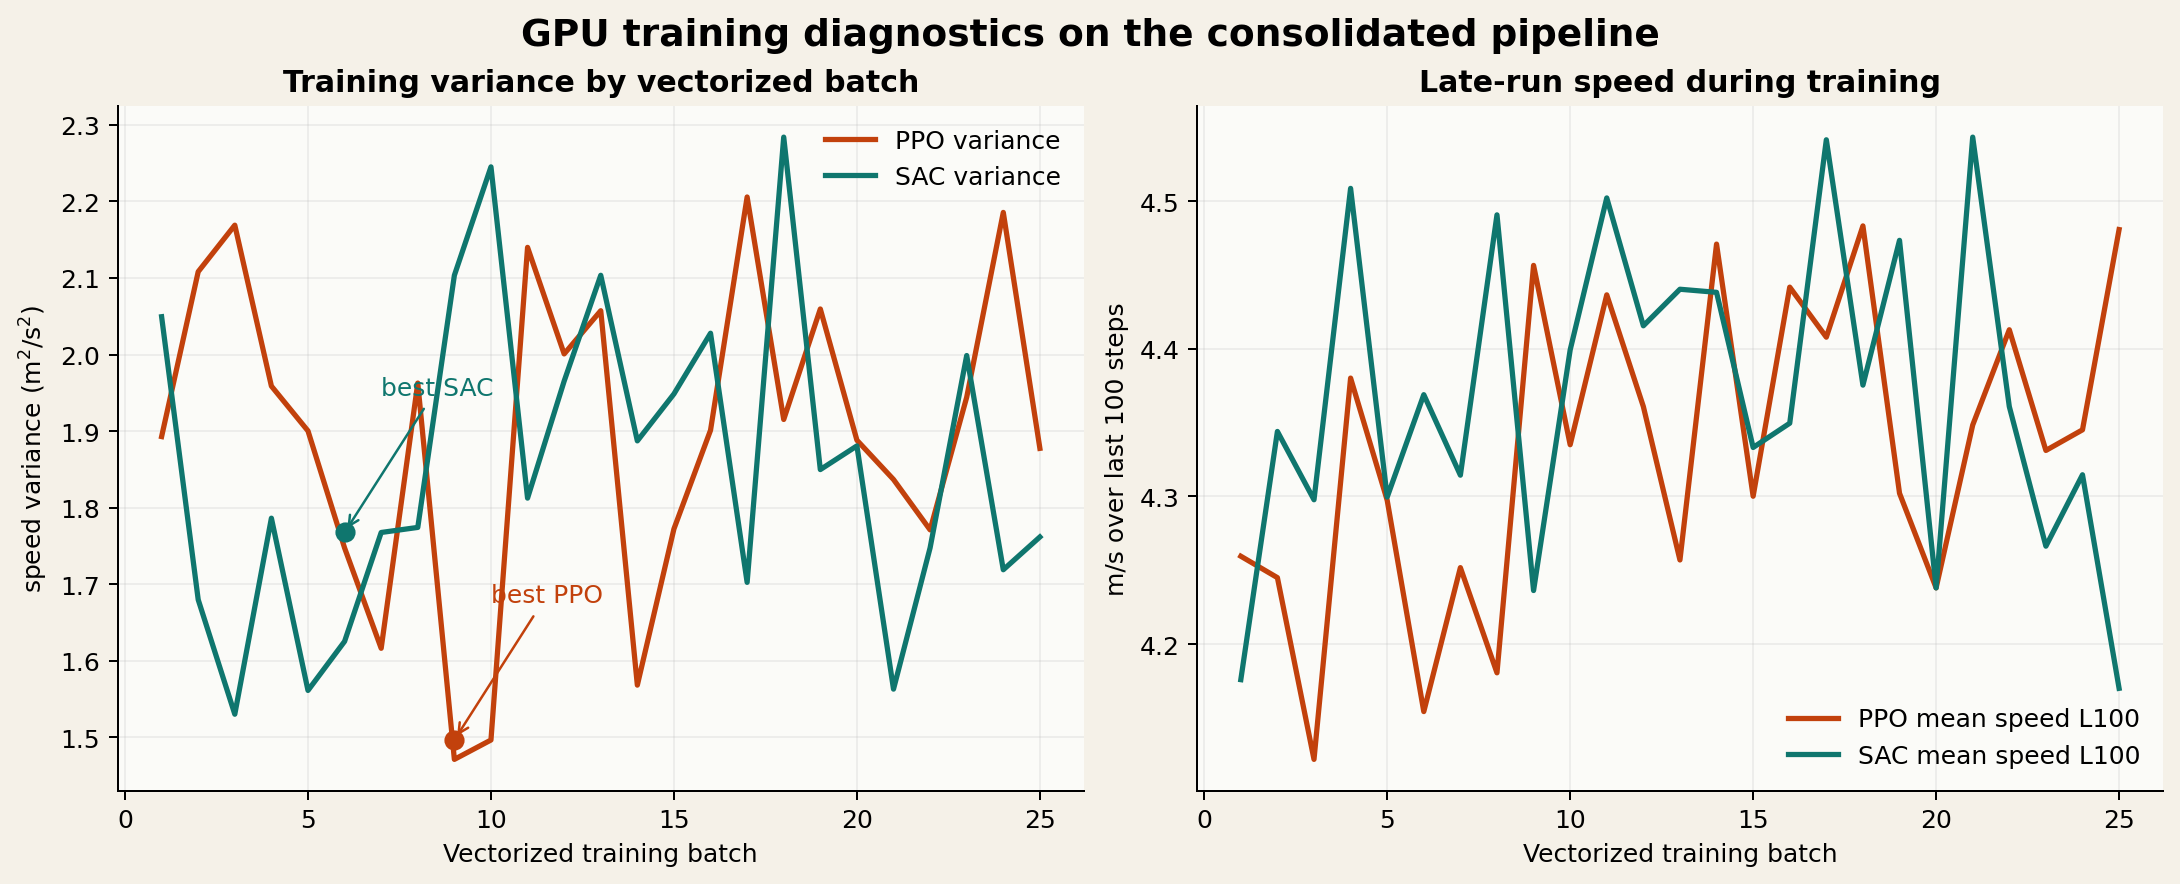
\includegraphics[width=\textwidth]{images/results/training_diagnostics.png}
    \caption{Training diagnostics from the final PPO and SAC runs. The horizontal axis counts vectorized batches, not single episodes; with 8 parallel environments, 25 batches correspond to 200 physical episodes.}
    \label{fig:training_diagnostics}
\end{figure}

Two remarks are worth emphasizing. First, PPO took noticeably longer than SAC in wall-clock time. This is expected in the current configuration because PPO performs many more optimizer updates per collected rollout batch, whereas SAC uses a smaller off-policy update loop. Second, the early-stopping monitor did not actually stop either run because the patience remained too large for a 25-batch training campaign. This is informative in itself: the monitoring logic is now present, but its configuration still needs to be tightened if it is to play a meaningful role.

\subsection{Evaluation results}

Table~\ref{tab:eval_results_updated} reports the final comparison across the three human-driver ratios. The most informative quantities are the late-run objective $\texttt{mean\_speed\_last100}$ and the late-run variance $\texttt{speed\_var\_last100}$, because they focus on the stabilized part of the trajectory rather than averaging the whole transient.

\begin{table}[!htbp]
\centering
\caption{Updated evaluation results for the consolidated pipeline.}
\label{tab:eval_results_updated}
\small
\resizebox{\textwidth}{!}{
\begin{tabular}{llccccccc}
\hline
HR & Method & Mean speed$_{100}$ & Var$_{100}$ & RMS acc. & RMS jerk & Min gap & Warnings & Clamps \\
 &  & (m/s) & (m$^2$/s$^2$) & (m/s$^2$) & (m/s$^3$) & (m) &  &  \\
\hline
\multirow{3}{*}{25\,\%}
 & No RL & \textbf{5.175} & 0.0098 & \textbf{0.578} & \textbf{8.682} & \textbf{0.510} & \textbf{0} & 3 \\
 & PPO   & 4.974 & 0.0185 & 0.679 & 10.334 & 0.510 & \textbf{0} & 3 \\
 & SAC   & 5.164 & \textbf{0.0063} & 0.635 & 9.632 & 0.510 & \textbf{0} & 3 \\
\hline
\multirow{3}{*}{50\,\%}
 & No RL & 4.716 & 1.142 & \textbf{0.437} & \textbf{5.169} & \textbf{0.510} & \textbf{0} & 3 \\
 & PPO   & 4.717 & 0.993 & 0.451 & 5.530 & \textbf{0.510} & \textbf{0} & 3 \\
 & SAC   & \textbf{4.719} & \textbf{0.968} & 0.454 & 5.577 & \textbf{0.510} & \textbf{0} & 3 \\
\hline
\multirow{3}{*}{75\,\%}
 & No RL & \textbf{2.887} & 3.718 & \textbf{0.420} & \textbf{3.451} & 0.307 & 42 & 4 \\
 & PPO   & 2.880 & \textbf{3.666} & 0.421 & 3.532 & \textbf{0.345} & 46 & \textbf{3} \\
 & SAC   & 2.866 & 3.777 & 0.424 & 3.531 & 0.300 & \textbf{39} & 5 \\
\hline
\end{tabular}
}
\end{table}

\begin{figure}[!htbp]
    \centering
    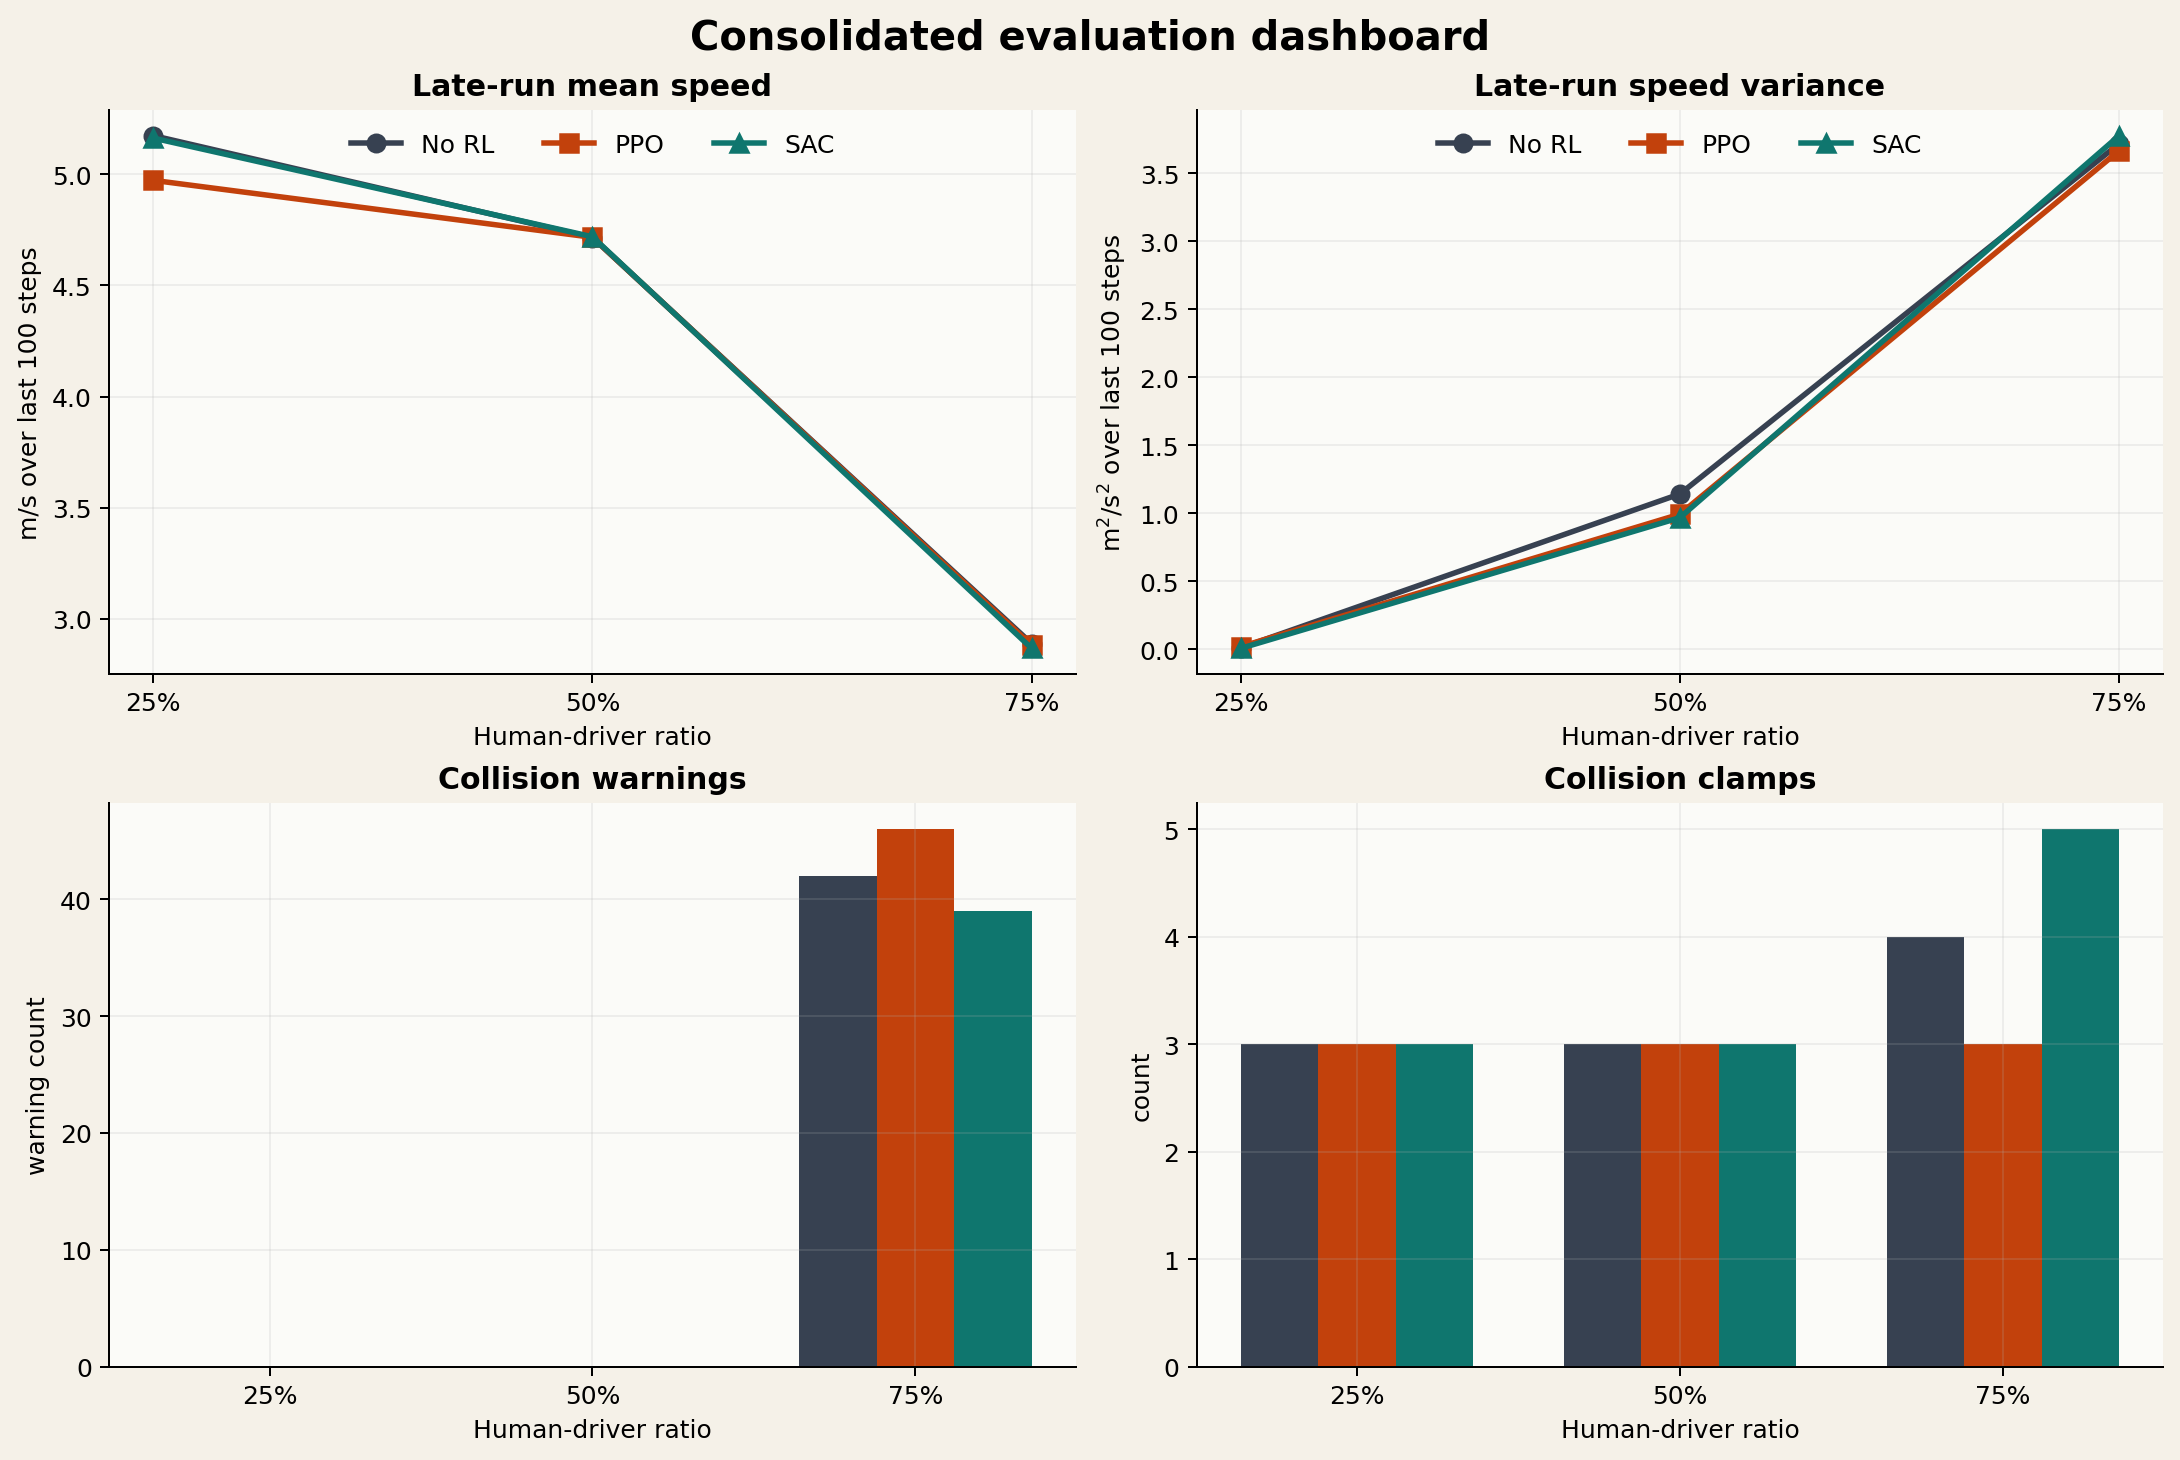
\includegraphics[width=\textwidth]{images/results/evaluation_dashboard.png}
    \caption{Self-contained evaluation dashboard stored locally in the report folder. The four panels show the main compromise between throughput, smoothness, collision warnings, and collision clamps.}
    \label{fig:evaluation_dashboard}
\end{figure}

\begin{figure}[!htbp]
    \centering
    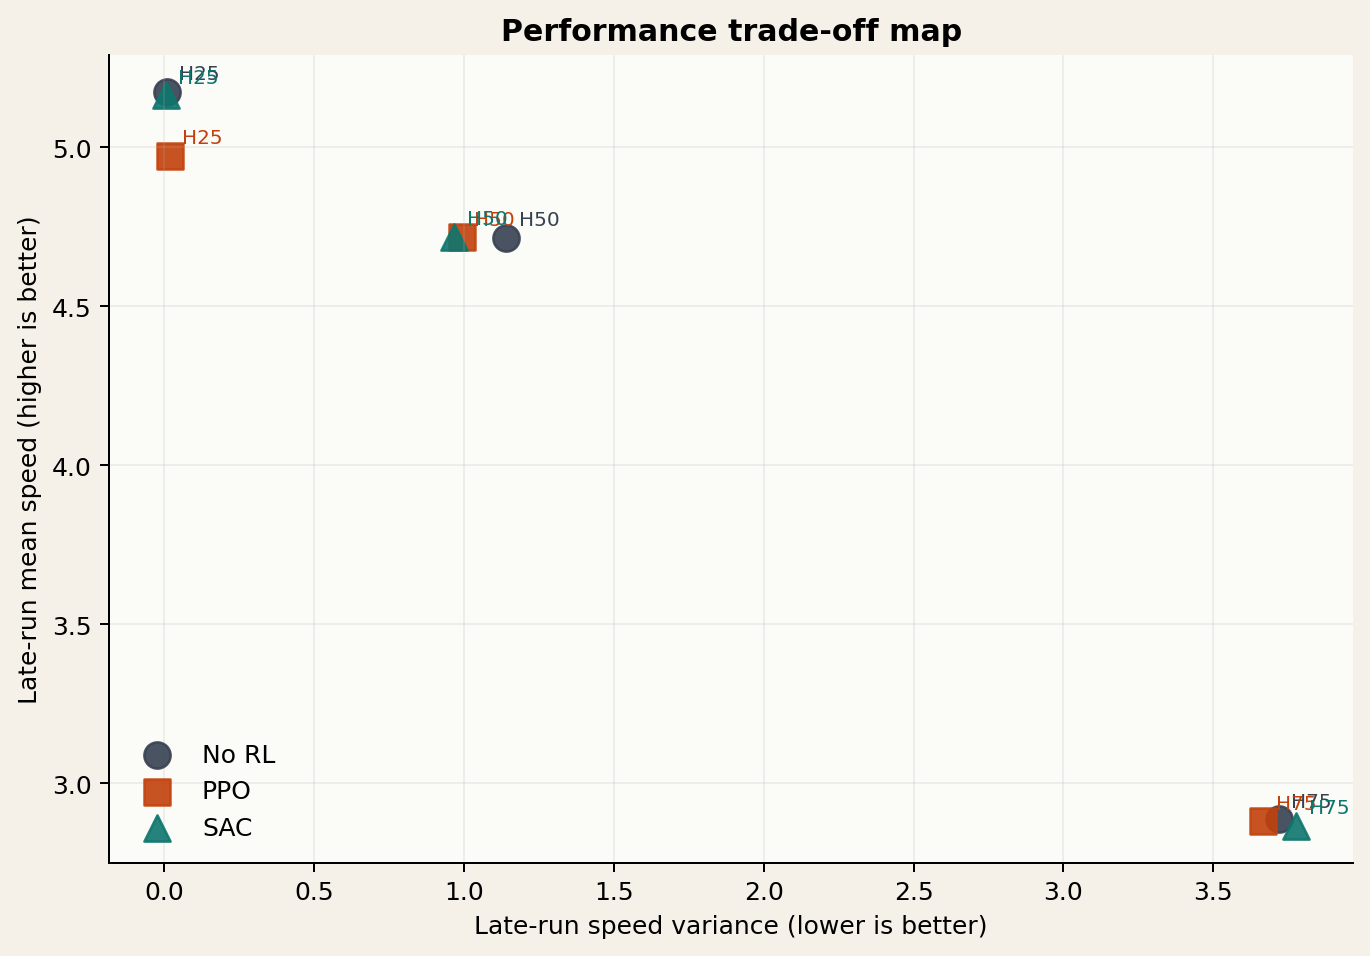
\includegraphics[width=0.82\textwidth]{images/results/performance_tradeoff_map.png}
    \caption{Trade-off map using late-run mean speed and late-run speed variance. The 50\,\% human-driver regime is the clearest region where learning improves the throughput--smoothness compromise.}
    \label{fig:tradeoff_map}
\end{figure}

\subsection{Reasoned interpretation}

Table~\ref{tab:qualitative_synthesis} summarizes the practical reading of the results. It is intentionally qualitative: the purpose is not to crown a universal winner, but to identify where each method is actually useful and where the current limitations remain dominant.

\begin{table}[!htbp]
\centering
\caption{Qualitative synthesis of the current results.}
\label{tab:qualitative_synthesis}
\small
\begin{tabular}{p{1.9cm}p{3.3cm}p{7.2cm}}
\hline
Regime & Current best reading & Main reason \\
\hline
25\,\% humans & No RL remains the strongest overall baseline & The traffic is already smooth; learning does not bring a meaningful throughput gain, and PPO even degrades comfort. SAC lowers variance slightly, but without a safety gain. \\
50\,\% humans & SAC has the best current compromise, with PPO close behind & This is the only regime where RL clearly improves late-run variance while preserving mean speed. The SAC run reduces late variance by about 15\,\% relative to No~RL. \\
75\,\% humans & No method is satisfactory yet & The regime remains dominated by safety events. PPO slightly improves variance and clamp count, SAC slightly reduces warning count, but every method still suffers collision clamps. \\
\hline
\end{tabular}
\end{table}

The main conclusion is that the 50\,\% human-driver regime is the real sweet spot of the current approach. At 25\,\%, the baseline controller is already so stable that learning has little room to help. At 75\,\%, the stochasticity introduced by the human-driven vehicles is strong enough that the learned residual policy still fails to make the system consistently safe. In between these two extremes, however, RL manages to reduce oscillations without sacrificing throughput, which is precisely the behavior the project aims to obtain.

Another important point is that all current runs fail the formal safety summary. This is not a bug in the evaluation code. The safety criterion checks both the minimum-gap threshold and the absence of collision clamps, and every run violated at least one of these conditions. The same observation explains why the string-stability amplification ratio is reported as invalid in the latest results: once collision clamps occur, the perturbation experiment is no longer a clean string-stability test.

\paragraph{A limitation that must be stated explicitly.}
The current results are based on a single random-seed evaluation campaign. They are therefore valid as matched-condition comparisons, but they are not yet sufficient to claim genuine generalization or to rule out over-training. The fact that both algorithms reached their best training variance early and then drifted away from it is a useful warning sign: longer training is not automatically better, and the next credible step is to evaluate the saved checkpoints on unseen seeds.

\paragraph{A remark I found particularly interesting.}
The most interesting pattern in these runs is that the learning signal seems to be genuinely informative only in the intermediate regime. This is a pleasant surprise from a traffic-flow point of view: the controller is not simply ``better everywhere'' or ``worse everywhere''. Instead, it helps most when the traffic is neither too easy nor too chaotic, which is exactly the kind of regime where hybrid control is supposed to matter.

\subsection{Future perspectives}

The most immediate next steps are now quite clear:
\begin{itemize}
    \item evaluate the selected PPO and SAC checkpoints on several unseen random seeds to check whether the observed gains at 50\,\% human drivers persist outside the current run;
    \item reduce the early-stopping patience to a value that makes sense for a 25-batch vectorized training campaign;
    \item enforce safety more directly during learning, for example with stronger hard constraints or constrained-RL formulations, because soft penalties alone are not preventing collision clamps in the difficult regimes;
    \item tune PPO and SAC differently instead of using almost parallel training budgets, since their optimization dynamics are not comparable in wall-clock time;
    \item extend training beyond a single human-driver ratio, either through curriculum training or mixed-ratio batches, in order to make the policy less specialized to the 50\,\% case.
\end{itemize}

At the present stage, the project already demonstrates a meaningful result: GPU-accelerated training makes larger experiments practical, and the learned residual controller can improve the throughput--smoothness trade-off in the intermediate mixed-traffic regime. The remaining challenge is no longer whether the idea can work at all, but how to make it robust and safe enough to support stronger scientific claims.

	
	\bibliography{references}
	
\end{document}
